\documentclass{article}
\usepackage{fontspec}
\defaultfontfeatures{Mapping=tex-text}
\usepackage{xunicode}
\usepackage{xltxtra}
\setmainfont{WenQuanYi Micro Hei Mono}
\usepackage[top=1.2in,bottom=1.2in,left=1.2in,right=1in]{geometry}
\usepackage[parfill]{parskip}
\usepackage{graphicx}
\usepackage{xcolor}
\usepackage{hyperref}
\usepackage{indentfirst}
%\setlength{\parindent}{2em}
\usepackage{listings}
\lstset{
    language=[ANSI]C,
    backgroundcolor=\color{lightgray},
    basicstyle=\footnotesize,
    numbers=left,
    numberstyle=\tiny,
    stepnumber=1,
    numbersep=5pt,
    breaklines=true,
    extendedchars=false,
    columns=flexible,
    showspaces=false,
    showstringspaces=false,
    %captionpos=b,
    %breakatwhitespace=false,
}

\usepackage[pagestyles]{titlesec}
\titleformat{\part}{\centering\Large\bfseries}{}{1em}{}
\titleformat{\section}{\large\bfseries}{\S\,\thesubsection}{1em}{}

\newcounter{RomanNumber}
\newcommand{\MyRoman}[1]{\setcounter{RomanNumber}{#1}\Roman{RomanNumber}}

\newpagestyle{main}{
\sethead{\small\S\,\thesection\quad\sectiontitle}{}{$\cdot$~\thepage~$\cdot$}
\setfoot{}{}{}\headrule}
\pagestyle{main}
\makeatletter

\renewcommand\paragraph{\@startsection{paragraph}{4}{\z@}{3.25ex \@plus1ex \@minus.2ex}{1.5ex \@plus.2ex}{\normalfont\normalsize\bfseries}}
\makeatother

\XeTeXlinebreaklocale "zh"
\XeTeXlinebreakskip = 0pt plus 1pt minus 0.1pt

\title{测量仪器的计算机控制}
\author{07300720027 马耀辉\\[2em]stesenchina@gmail.com}
\begin{document}
\maketitle

%\newpage
%\tableofcontents
%\newpage

\section{目标}
1. 实现虚拟仪器的计算机控制.\\
2. 利用B/S模式实现对仪器的远程控制.\\

\section{开发环境}
\subsection{硬件}
\parbox[t]{4cm}{
测量仪器\\
}
\parbox[t]{12cm}{
Fluke 45\\
}

\subsection{软件}
\parbox[t]{4cm}{
编辑器\\
编译器\\
解析器\\
中文编码\\
}
\parbox[t]{12cm}{
Vim + ctag\\
gcc-4.4.5\\
Bash-4.1.5, perl-5.10.1, Octave-3.2.4\\
UTF-8\\
}

\section{设计}
随着虚拟仪器技术的提高和B/S计算模式的成熟, 我为本次实验设计了一个基于B/S模式的虚拟仪器控制方式:\\
\begin{center}
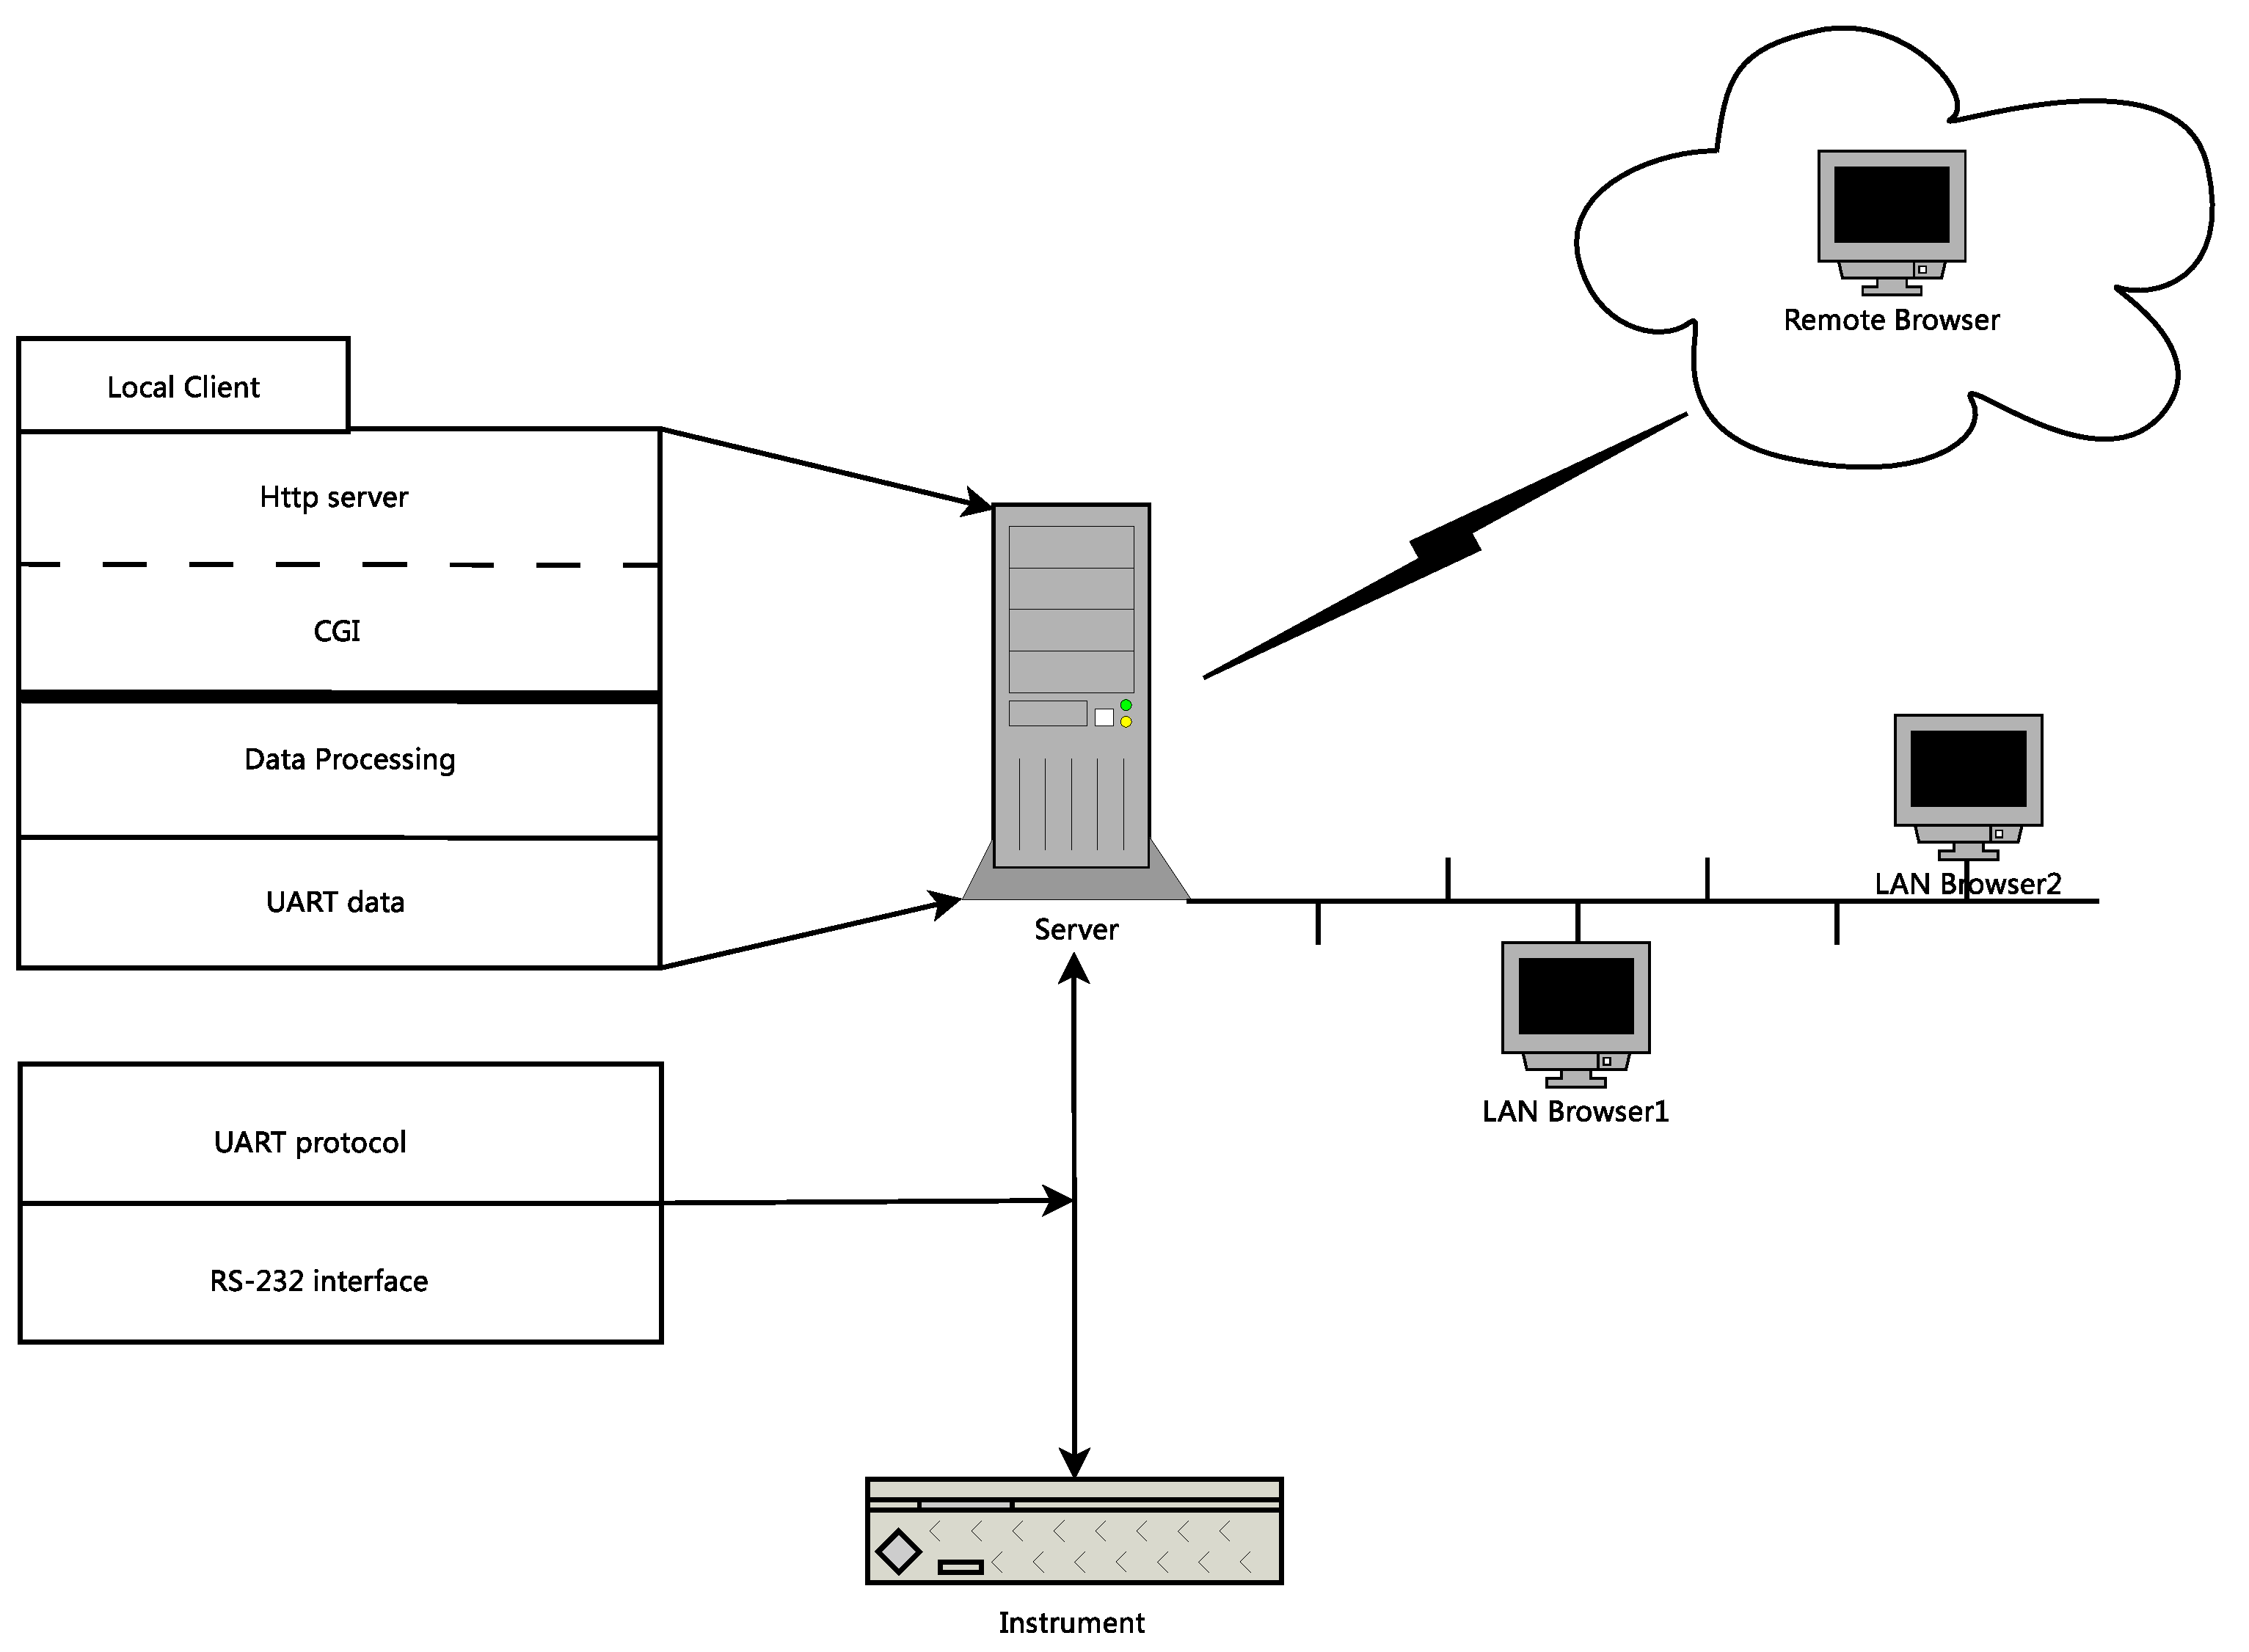
\includegraphics[width=\textwidth]{image/all.eps}\\[2em]
\end{center}
主机端通过串口获取仪器数据, 将数据经过处理后, 提供Web服务, 实现远程的控制和测量, 同时主机端也可以通过本地浏览器获取仪器数据.\\
\section{实现}
整个系统的实现分为两部分: browser端和server端.

\subsection{browser实现}
browser端用任何一个标准web浏览器替代即可.\\
为了系统的完整性, 我设计了一个基于QT4/Webkit的简单的浏览器, 用于为整个系统提供本地的GUI界面.

\subsection{server实现}
server端分为如下几个层次, 每层从下层获取数据, 并向上层提供服务:\\
\begin{center}
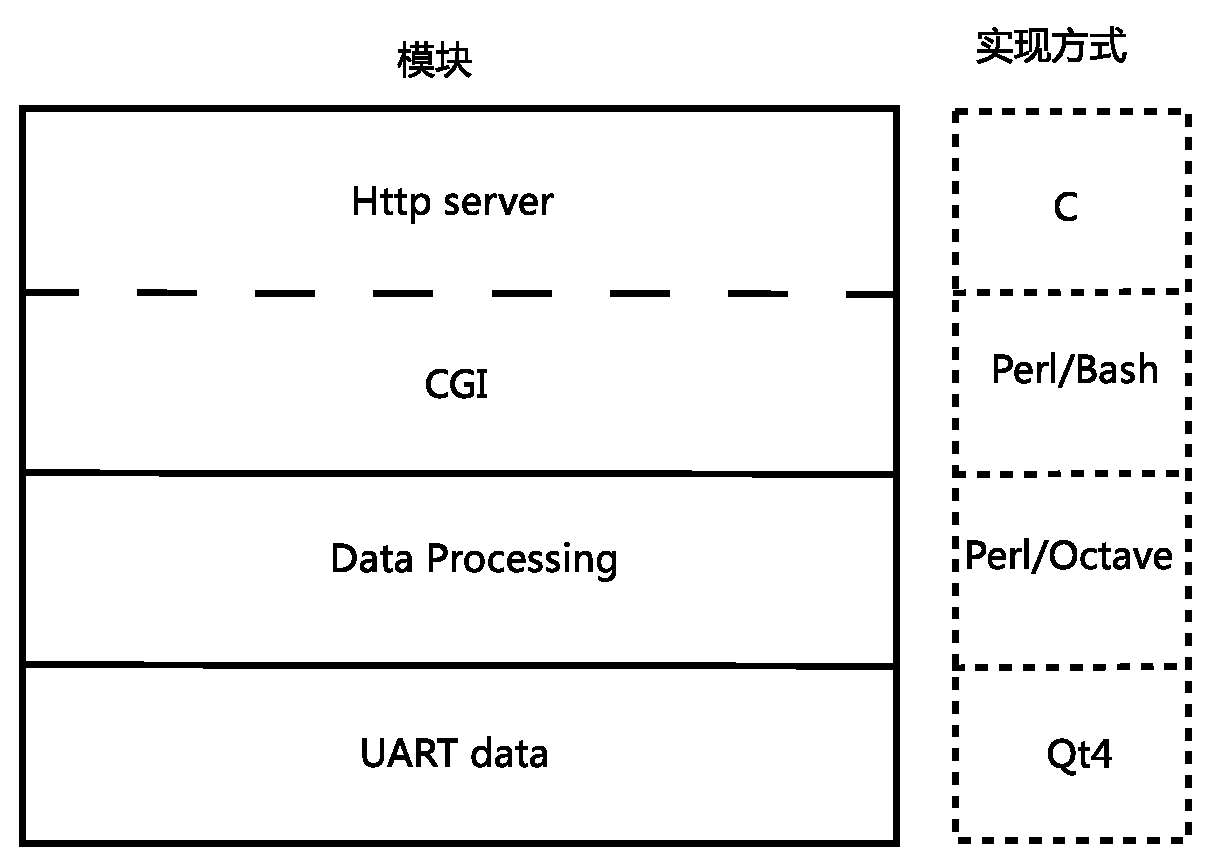
\includegraphics[width=0.5\textwidth]{image/server.eps}\\[2em]
\end{center}
1. 串口数据层负责向串口发送命令, 并读取测量数据, 打印在STDOUT上.\\
2. 数据处理层负责从标准输出上获取数据, 取出有效信息, 存入ASCII格式的数据文件, 然后调用Octave(也可以是Matlab, 两者语法兼容)对数据进行处理, 处理结果保存为ASCII格式的数据文件, 以及png格式图片.\\
3. CGI层从属于Http服务器层, 作为它的一部分, 用于读取用户请求, 然后调用数据处理层, 并向其传递参数, 它是对数据处理层的封装, 向Http服务器层提供统一的接口.\\
4. Http服务器层负责提供web服务, 其中html文件中会调用刚才处理好的数据和图片文件.\\[2em]
具体的实现:\\
1. 串口数据层可以用C/C++/Shell/Perl等语言实现, 原理都是通过操作linux下的设备节点文件/dev/ttyUSB0(第0个usb串口), QT提供的串口库可以很好的解决串口阻塞问题, 性能比较稳定, 所以选择C++作为最底层的实现.\\
2. 数据处理层用于解析标准输出, 进行运算并画出图像. 它需要强大的正则表达式以及数学运算和信号处理能力, 并且需要很好的可扩展性, 用于对多样化数据的处理. 所以用Perl实现数据解析, 用Octave进行数据处理. 这样可以缩减开发调试成本, 并且提供了丰富的数学函数库, 像卷积,相关,傅立叶变换,数字滤波器等等, 在数字信号处理方面, 它可以提供比Labview更强大的功能.\\
3. CGI运行于服务器上, 主要工作是调用服务器端的文件或程序, 所以用Shell或者Perl语言实现.\\
4. Http服务器层可以用现有的支持cgi的服务器软件代替, 比如主流的Apache, lighttpd等, 但为了实现整个系统的统一性, 我用c语言实现了一个最简单的支持cgi的http服务器. 代码部分来自上学期计算机网络的作业, 主要参考webfs\cite{webfs}项目\\

\section{成果}
通过对每个模块的调试, 到整个系统的调试, 最终整个测量仪器计算机控制系统能够正常运行, 可以在本地或者远程通过web方式, 控制和读取Fluke数字万用表的测量数据, 并且能提供一些基本的数据处理能力: 均值,方差,自相关,傅立叶变换等.\\
\begin{center}
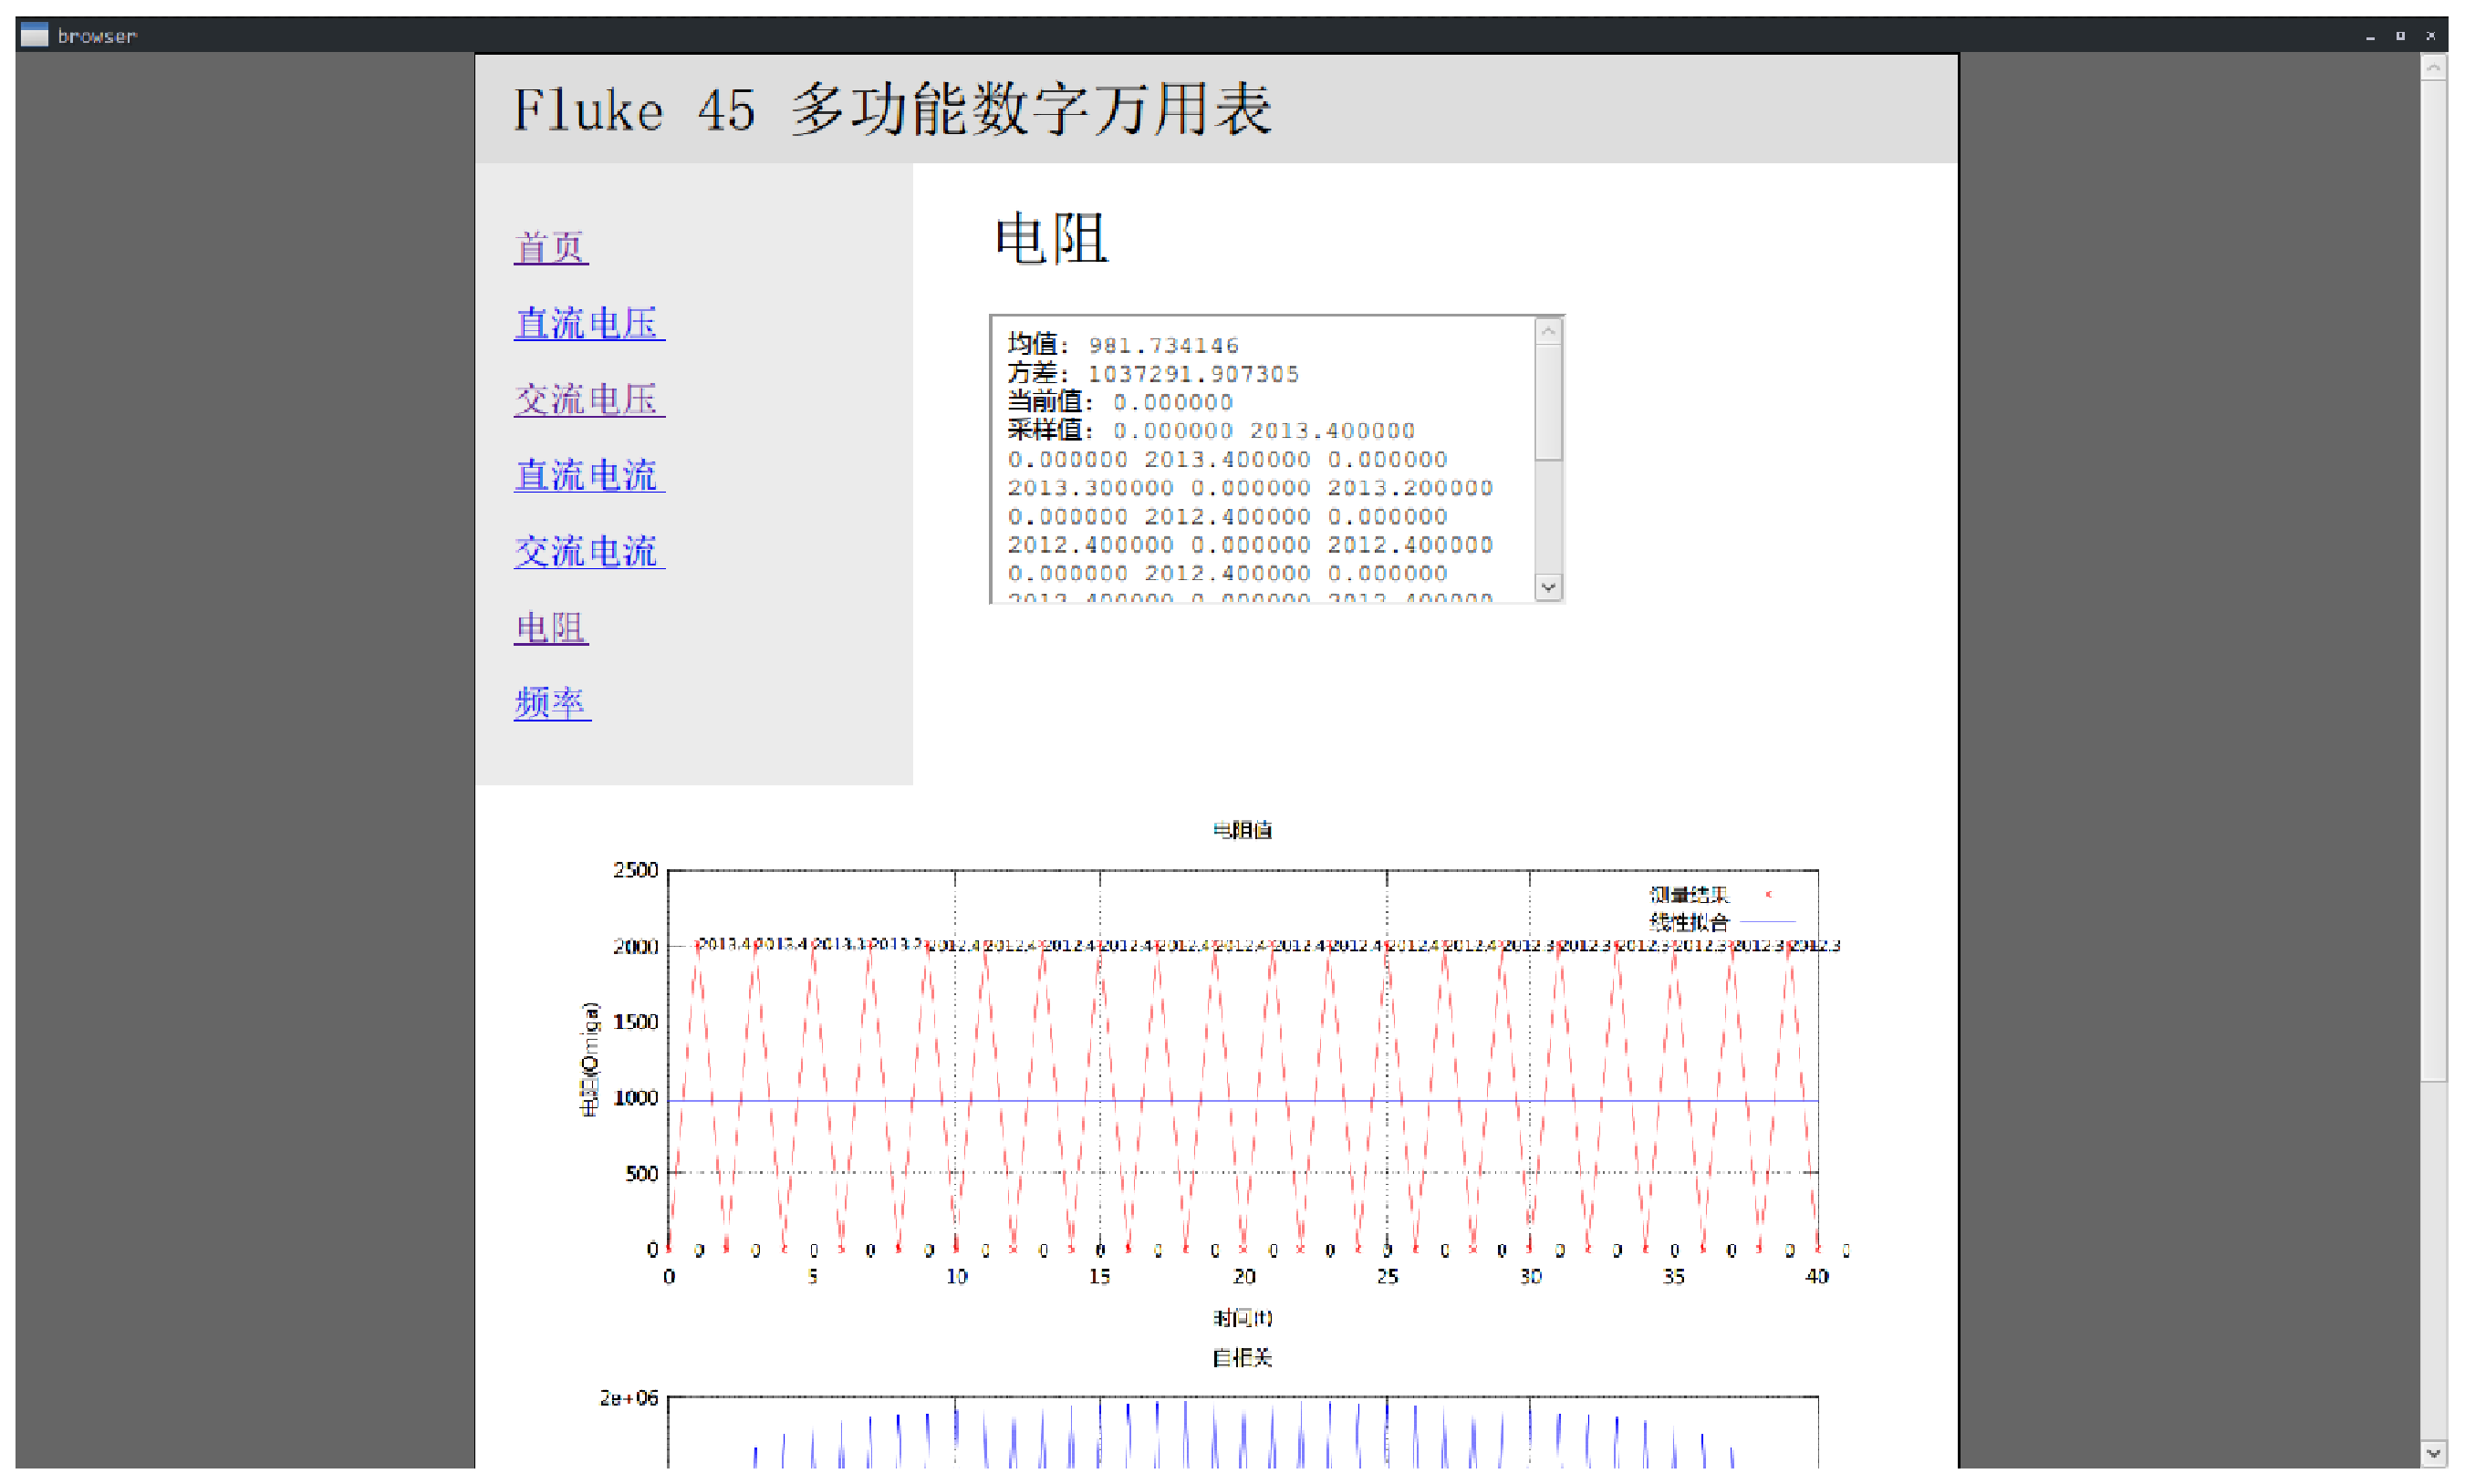
\includegraphics[width=0.8\textwidth]{image/localui1.eps}\\
本地界面\\[2em]
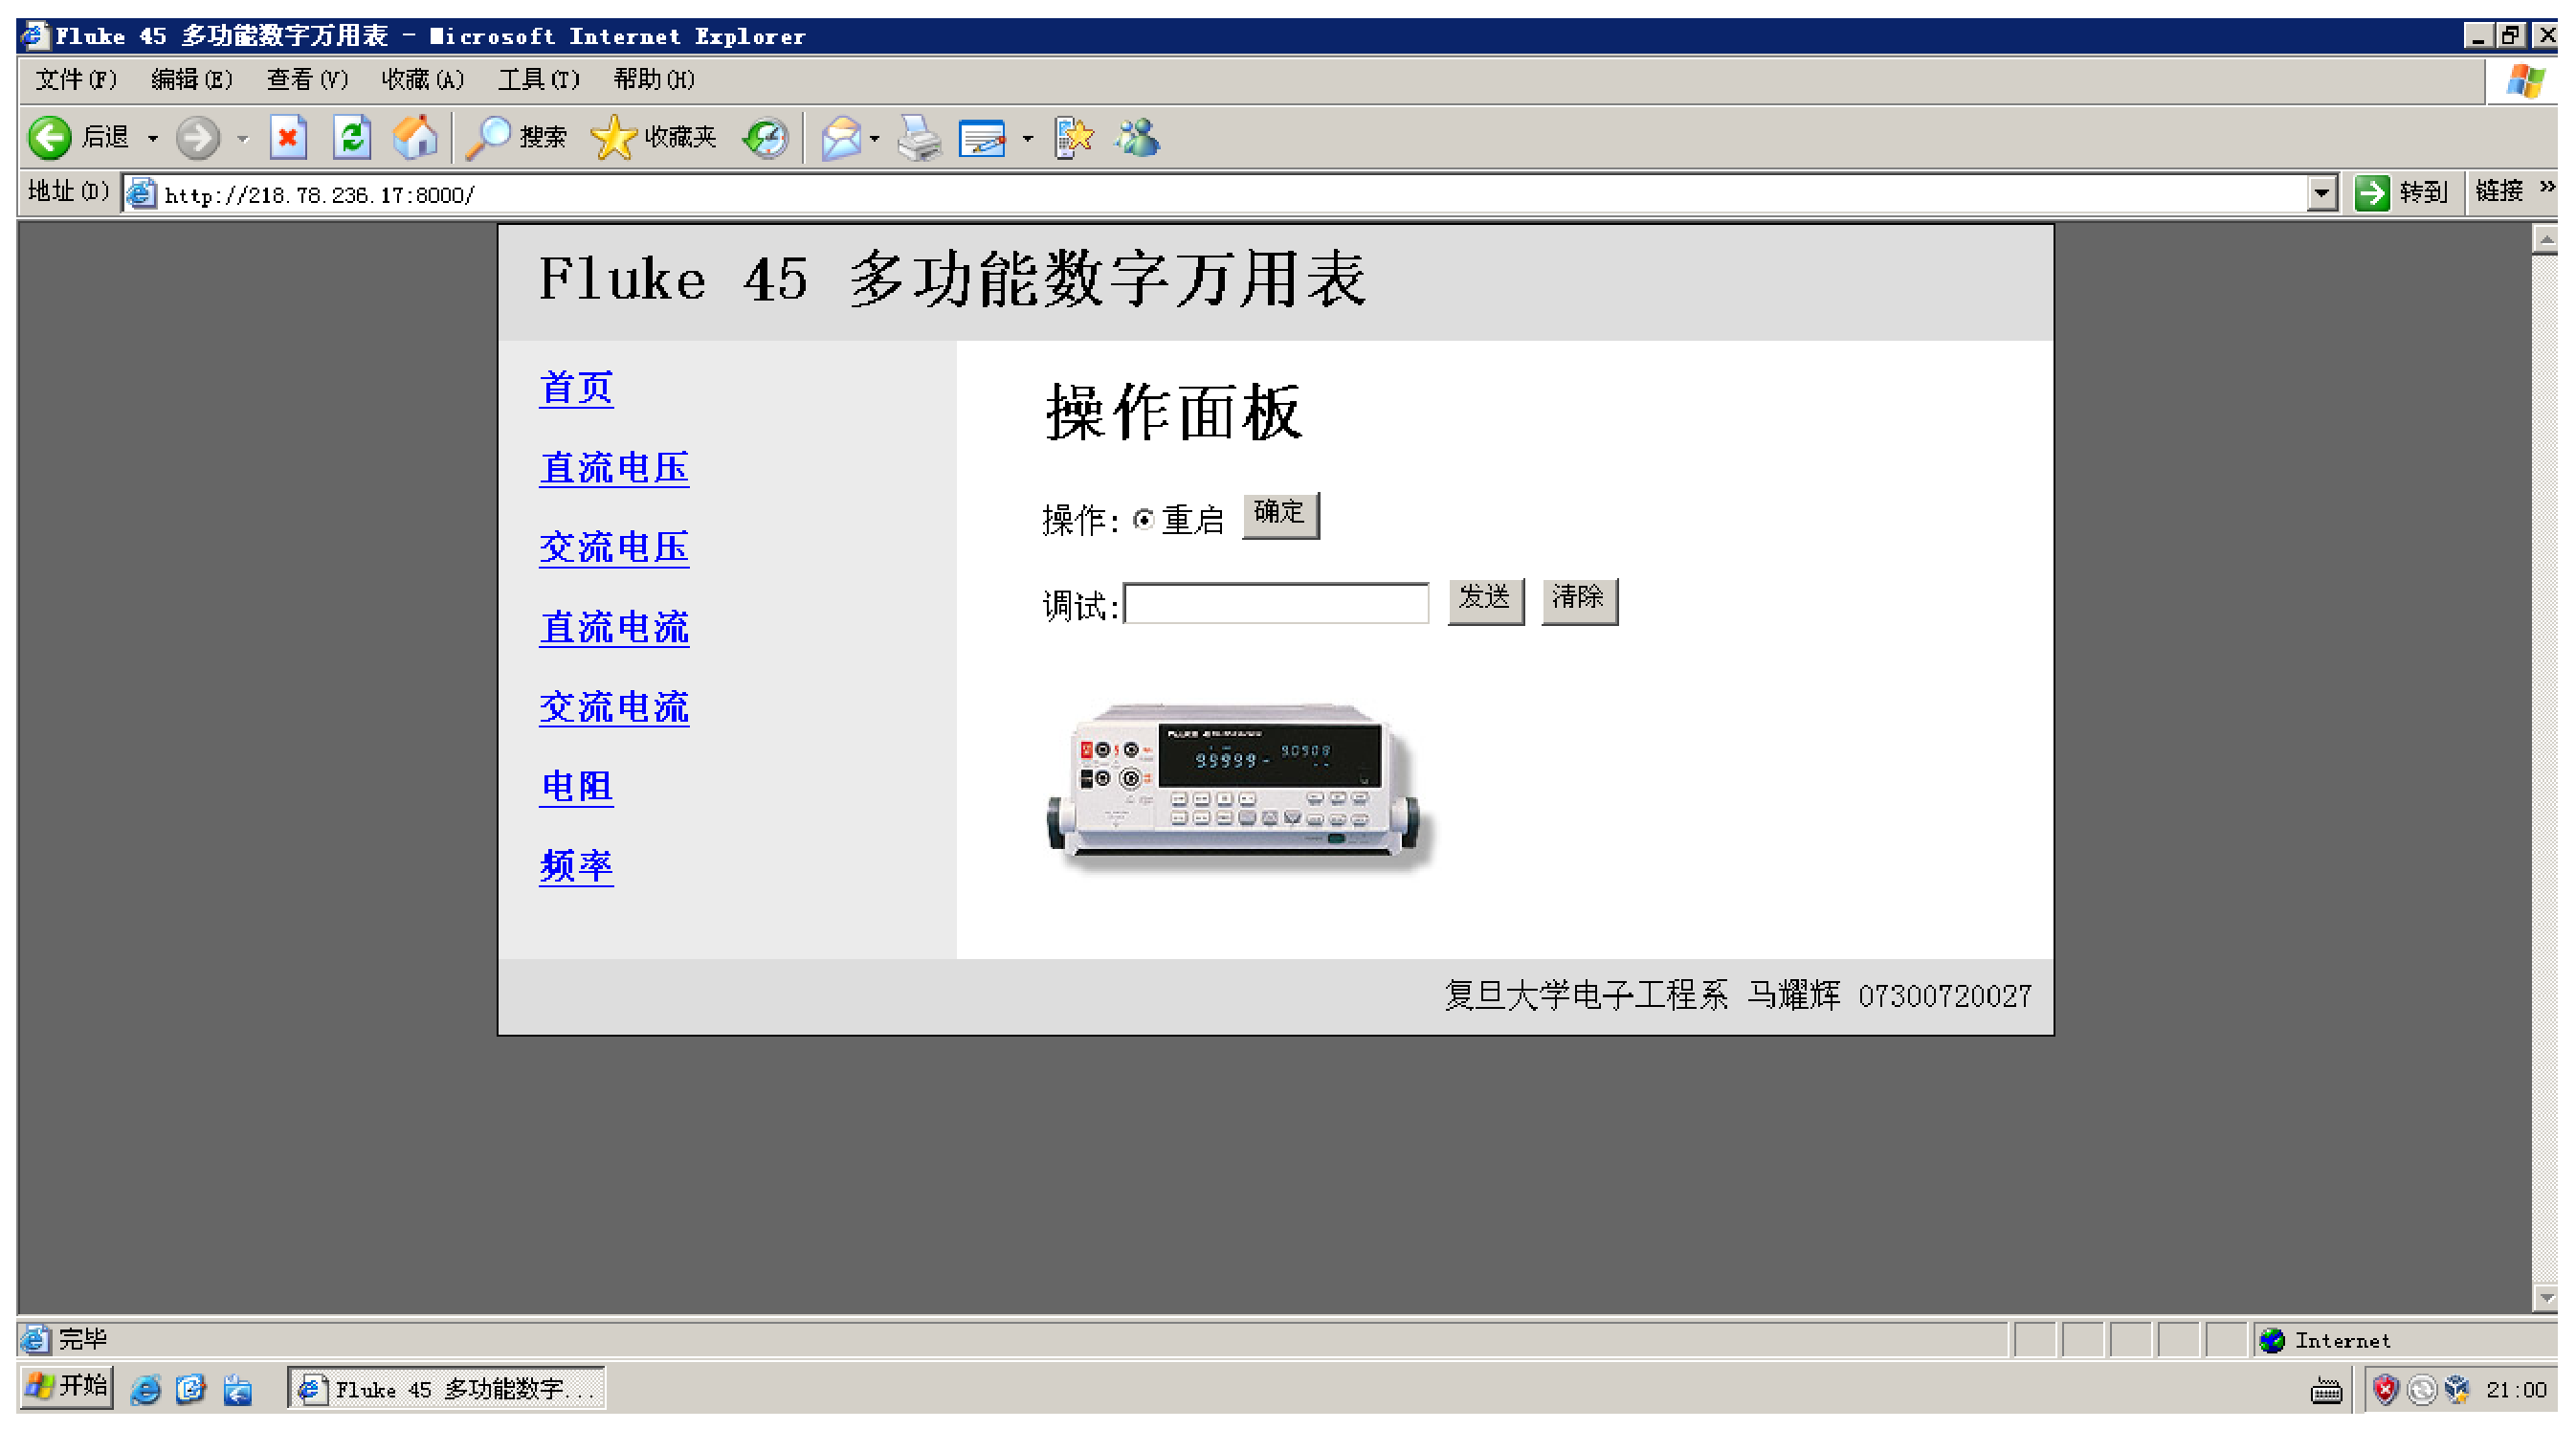
\includegraphics[width=0.8\textwidth]{image/remoteui.eps}\\
远程标准浏览器界面\\[2em]
\end{center}
这个系统的缺陷是:\\
1. 跨平台能力比较弱, 严重依赖Unix类操作系统, server端无法直接移植到Windows平台.\\
2. 整个系统的各个模块通过Shell和Perl脚本相互调用, 开启多个进程, 开销比较高, 数据传递效率比较低, 多个客户端频繁调用会严重影响系统负载. 应当用线程的方式来代替.\\
3. 串口读写模块用Qt实现, 需要X-window或Framebuffer图形支持, 难以部署到不集成图形系统的服务器上.\\
4. 没有实现插件功能, 添加新的cgi程序需要修改大量html文件, 系统越复杂, 这个缺点越明显.\\[2em]

所有的代码(包括本实验报告)全部放在github网站上, 通过如下方式获取:\\
\begin{lstlisting}
git clone git://github.com/stesen/vi.git
\end{lstlisting}
\section{总结}
通过本次实验, 加深了对虚拟仪器技术和B/S计算模式的理解, 熟悉了项目的设计-开发-测试的流程.
\bibliographystyle{plain}
\bibliography{ref}

\end{document}
